% Geometry taken directly from my lectures notes on tight binding in graphene
\newcommand{\alat}{1 cm}
\newcommand{\sqth}{1.73205080757}
\newcommand{\Klen}{2 cm}
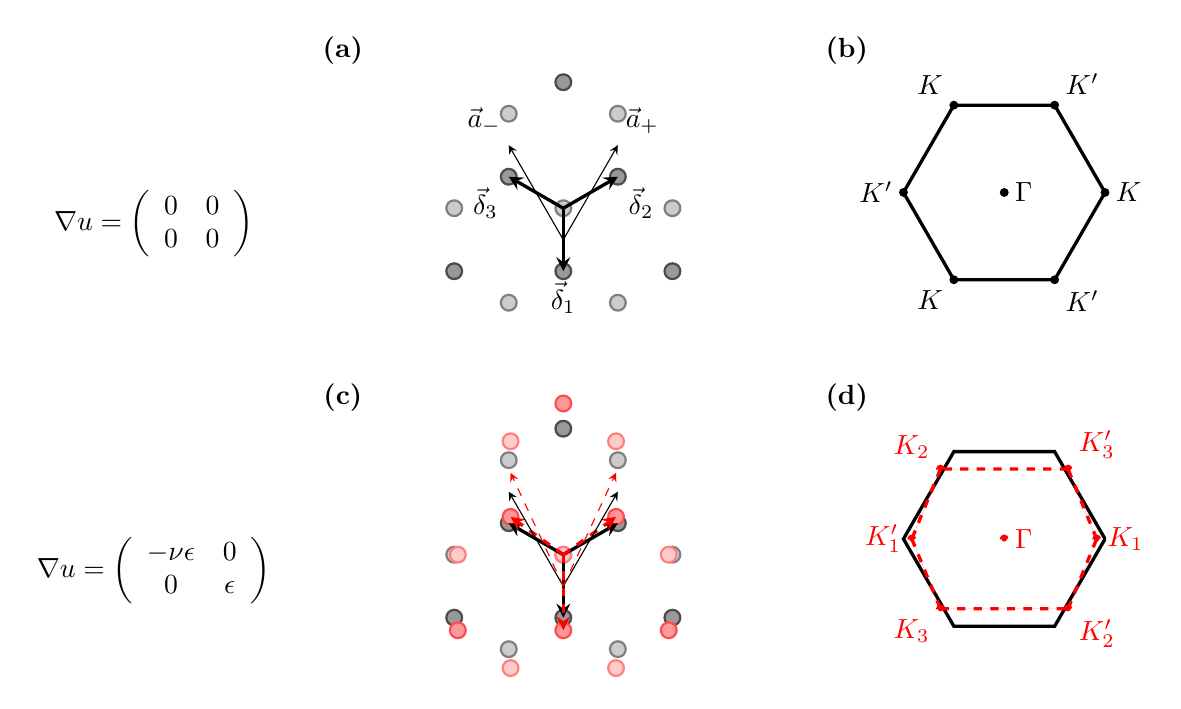
\begin{tikzpicture}[>=stealth,scale=.8,
		nnarrow/.style={color=black,very thick, ->},					% Nearest neighbor vectors
		nnarrows/.style={color=red,very thick, dashed, ->},				% Strained nearest neighbor vectors		
		lvarrow/.style={color=black, ->},								% lattice vector unstrained
		lvarrows/.style={color=red, dashed, ->},						% Lattice vector strained
		BZ/.style={color=black,fill=black,very thick},					% Unstrained BZ lines
		BZs/.style={color=red,fill=red,dashed, very thick},				% Strained BZ lines
		circ2/.style={radius=1.5pt},									% Dots at K points on BZ
		A/.style={circle,draw=black!50,fill=black!20,
			thick,minimum size=2 mm,inner sep=0pt}, 					% A sublattice dots (unstrained)
		As/.style={circle,draw=red!50,fill=red!20,
			thick,minimum size=2 mm,inner sep=0pt}, 					% A sublattice dots (strained)
		B/.style={circle,draw=black!70,fill=black!40,
			thick,minimum size=2mm,inner sep=0pt},						% B sublattice dots (strained)
		Bs/.style={circle,draw=red!70,fill=red!40,
			thick,minimum size=2mm,inner sep=0pt}]						% B sublattice dots (unstrained)					

	% Graphene lattice, sublattices different colors, nearest neighbor vectors and lattice vectors
	\begin{scope}[xshift=-3.5 cm,yshift=1.5 cm]				% Lattice vector arrows

		%This scope is clipped to limit the drawn lattice to a square
		\clip (-2.75cm,-2cm) rectangle(2.75cm,2.75cm);
		% \draw (-2.75cm,-2cm) rectangle(2.75cm,2.75cm);

		% Draw the unstrained lattice
		\foreach \ip in {-1,0,...,1}
			\foreach \im in {-1,0,...,1}
			{
			\node at (\ip*\sqth*\alat/2-\im*\sqth*\alat/2, \ip*\alat*3/2+\im*\alat*3/2      ) [A] {};
			\node at (\ip*\sqth*\alat/2-\im*\sqth*\alat/2, \ip*\alat*3/2+\im*\alat*3/2-\alat) [B] {};
			}

		% Draw the nearest neighbor vectors
		\draw[nnarrow] (0,0) -- +(270:\alat) node[anchor=north     ]{$\vec{\delta}_1$};
		\draw[nnarrow] (0,0) -- +( 30:\alat) node[anchor=north west]{$\vec{\delta}_2$};
		\draw[nnarrow] (0,0) -- +(150:\alat) node[anchor=north east]{$\vec{\delta}_3$};
		
		% Draw the lattice vectors
		\draw[lvarrow] (0,-\alat/2) -- +( 60:\sqth*\alat)node[circle,anchor=south west]{$\vec{a}_+$};
		\draw[lvarrow] (0,-\alat/2) -- +(120:\sqth*\alat)node[circle,anchor=south east]{$\vec{a}_-$};
	\end{scope}

	% Reciprocal space BZ and high symmetry points
	\begin{scope}[xshift=3.5cm,yshift=1.75 cm,scale=.8]

		% Draw the BZ
		\draw[BZ]
			(  0:\Klen) circle[circ2] node[anchor=west      ]{$\bm{K} $} --
			( 60:\Klen) circle[circ2] node[anchor=south west]{$\bm{K'}$} --
			(120:\Klen) circle[circ2] node[anchor=south east]{$\bm{K }$} -- 
			(180:\Klen) circle[circ2] node[anchor=east      ]{$\bm{K'}$} -- 
			(240:\Klen) circle[circ2] node[anchor=north east]{$\bm{K }$} -- 
			(300:\Klen) circle[circ2] node[anchor=north west]{$\bm{K'}$} -- 
			(  0:\Klen);

		% Label the high symmetry points
		\draw[BZ] (0,0) circle[circ2] node[anchor=west]{$\Gamma$};
	\end{scope}

	% Strained lattice
	\begin{scope}[xshift=-3.5 cm,yshift=-4 cm]
		%This scope is clipped to limit the drawn lattice to a square
		\clip (-2.75cm,-2cm) rectangle(2.75cm,2.75cm);
		% \draw (-2.75cm,-2cm) rectangle(2.75cm,2.75cm);

		% Draw the unstrained lattice
		\foreach \ip in {-1,0,...,1}
			\foreach \im in {-1,0,...,1}
			{
			\node at (\ip*\sqth*\alat/2-\im*\sqth*\alat/2, \ip*\alat*3/2+\im*\alat*3/2      ) [A] {};
			\node at (\ip*\sqth*\alat/2-\im*\sqth*\alat/2, \ip*\alat*3/2+\im*\alat*3/2-\alat) [B] {};
			}

		% Draw the strained lattice
		\foreach \ip in {-1,0,...,1}
			\foreach \im in {-1,0,...,1}
			{
			\node at (\ip*.837*\alat-\im*.837*\alat, \ip*\alat*1.8+\im*\alat*1.8          ) [As] {};
			\node at (\ip*.837*\alat-\im*.837*\alat, \ip*\alat*1.8+\im*\alat*1.8-1.2*\alat) [Bs] {};
			}

		% Draw the unstrained nearest neighbor vectors
		\draw[nnarrow] (0,0) -- +(270:\alat);
		\draw[nnarrow] (0,0) -- +(30 :\alat);
		\draw[nnarrow] (0,0) -- +(150:\alat);

		% Draw the strained nearest neighbor vectors
		\draw[nnarrows] (0,0) -- +(    0*\alat,-1.2*\alat);
		\draw[nnarrows] (0,0) -- +( .837*\alat, .60*\alat);
		\draw[nnarrows] (0,0) -- +(-.837*\alat, .60*\alat);

		% Draw the unstrained lattice vectors
		\draw[lvarrow] (0,-\alat/2) -- +( 60:\sqth*\alat);
		\draw[lvarrow] (0,-\alat/2) -- +(120:\sqth*\alat);

		% Draw the strained lattice vectors
		\draw[lvarrows] (0,-\alat/2) -- +( .837*\alat,1.8*\alat);
		\draw[lvarrows] (0,-\alat/2) -- +(-.837*\alat,1.8*\alat); 
	\end{scope}

	% Strained BZ
	\begin{scope}[xshift=3.5 cm,yshift=-3.75 cm,scale=.8]
		% Draw the unstrained BZ
		\draw[color=black,very thick]
			(  0:\Klen)  --
			( 60:\Klen)  --
			(120:\Klen)  -- 
			(180:\Klen)  -- 
			(240:\Klen)  -- 
			(300:\Klen)  -- 
			(  0:\Klen);

		% Draw the strained 
		\draw[BZs]
			( .917*\Klen, .000*\Klen) circle[circ2] node[anchor=west      ]{$\bm{K_1} $} --
			( .633*\Klen, .693*\Klen) circle[circ2] node[anchor=south west]{$\bm{K_3'}$} --
			(-.633*\Klen, .693*\Klen) circle[circ2] node[anchor=south east]{$\bm{K_2}$} -- 
			(-.917*\Klen, .000*\Klen) circle[circ2] node[anchor=east      ]{$\bm{K_1'}$} -- 
			(-.633*\Klen,-.693*\Klen) circle[circ2] node[anchor=north east]{$\bm{K_3}$} -- 
			( .633*\Klen,-.693*\Klen) circle[circ2] node[anchor=north west]{$\bm{K_2'}$} -- 
			( .917*\Klen, .000*\Klen);

		% Label the high symmetry points
		\draw[BZs] (0,0) circle[circ2] node[anchor=west]{$\Gamma$};
	\end{scope}


	% (a) (b) (c) and (d) labels
	\node at (-7cm,4cm)   {\textbf{(a)}};
	\node at ( 1cm,4cm)   {\textbf{(b)}};
	\node at (-7cm,-1.5cm){\textbf{(c)}};
	\node at ( 1cm,-1.5cm){\textbf{(d)}};

	% Strain labels on the right side
	\node at (-10cm, 1.25 cm) {$\bm{\nabla u}=\left(\begin{array}{cc} 0 & 0 \\ 0 & 0 \end{array}\right)$};
	\node at (-10cm,-4.25 cm) {$\bm{\nabla u}=\left(\begin{array}{cc} -\nu \epsilon & 0 \\ 0 & \epsilon \end{array}\right)$};
\end{tikzpicture}